\chapter{Reproducibility}
\label{app:repro}

\section{Repository layout}

{\footnotesize
\begin{verbatim}
parkinson-domain-shift/
  data/raw/archives/     SisFall_dataset.zip, Daphnet_dataset.zip (untouched)
  data/processed/        windows in g, metadata, scalers, PyTorch tensors
  notebooks/             01-07, executed, with outputs
  src/                   models, training loop, metrics, transforms
  models/<arch>/seed<k>.pt   checkpoints with config, scaler and threshold
  results/figures/       every figure of this report (PNG and PDF)
  results/metrics/       every table of this report (CSV/JSON)
  results/confusion_matrices/
  paper/                 this report and the poster (LaTeX + PDF)
\end{verbatim}
}

\section{Running the pipeline}

The notebooks are executed in order. Notebooks 01, 02, 06 and 07 take a few minutes; 03--05 train
neural networks and are the only expensive steps. Notebooks 03 and 05 write their results row by
row and skip finished runs when restarted, and notebook 04 reloads existing checkpoints, so an
interrupted run can be resumed. The training notebooks were executed on a Colab T4 GPU with
\texttt{colab/RUN\_ON\_COLAB.ipynb}; notebooks 04, 06 and 07 were then re-executed on CPU from the
saved checkpoints (inference only), which reproduced all metrics to four decimals.

\section{Design decisions and the shortcuts they avoid}

\begin{table}[ht]
\centering
\small
\begin{tabular}{p{3.6cm}p{4.4cm}p{5.2cm}}
\toprule
Aspect & Common shortcut & This study \\
\midrule
Fall labels & every window of a fall file & windows centred on the impact ($\pm0.5$\,s), ambiguous ones dropped \\
Sensors & whatever channels are available in each dataset & one waist/trunk accelerometer in both domains, in a V/AP/ML frame \\
Sampling rate & target upsampled to the source rate & source downsampled to 64\,Hz (anti-aliased) \\
Units & raw counts / mg, then z-scored & $g$ in both domains \\
Target windows & across concatenated recordings & inside contiguous valid segments; dropouts removed \\
Scaling & mean / standard deviation & robust (median/IQR), three label-free target variants \\
Training & tuned separately for each model & identical loss, optimiser, batches, seeds and budget \\
Threshold & fixed by hand & $F_2$-optimal on source validation \\
\bottomrule
\end{tabular}
\caption{Design decisions of this study and the simpler choices they replace.}
\label{tab:changes}
\end{table}

\section{Additional figures}

\begin{figure}[H]
\centering
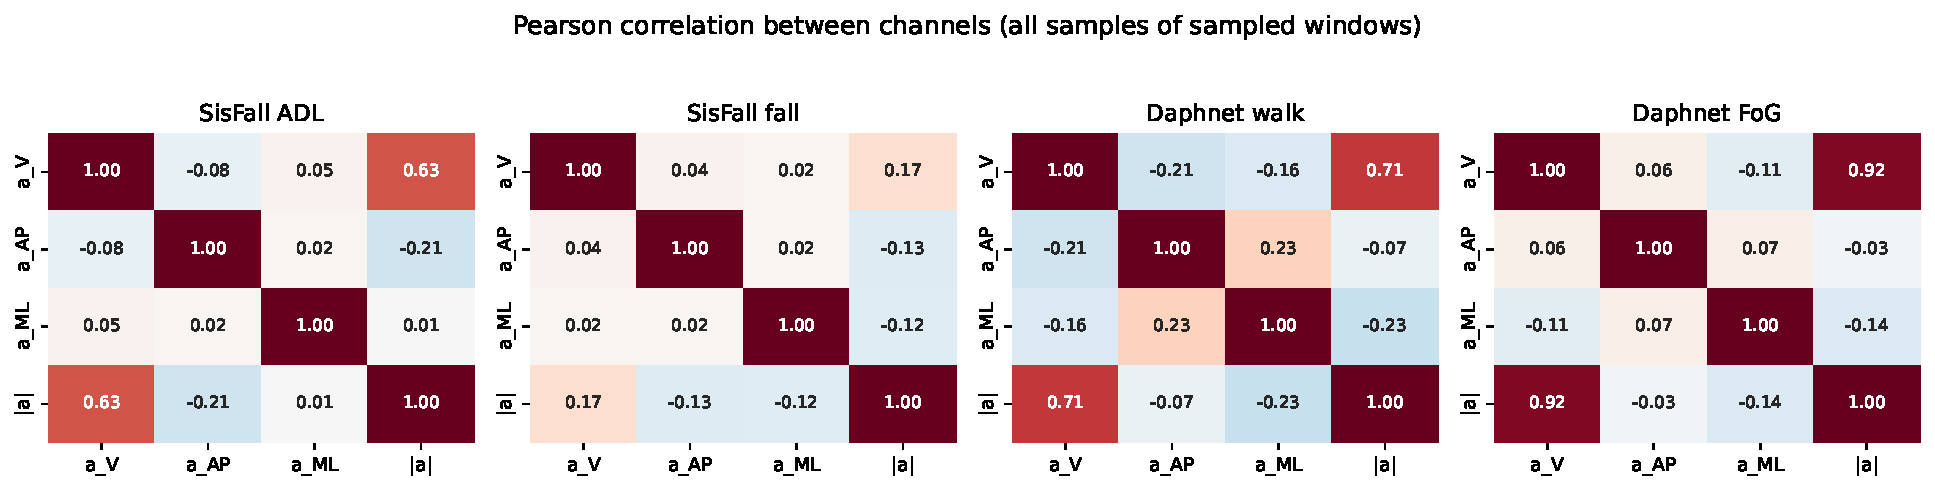
\includegraphics[width=\textwidth]{fig09_channel_correlation}
\caption{Pearson correlation between the four channels, per group.}
\end{figure}

\begin{figure}[H]
\centering
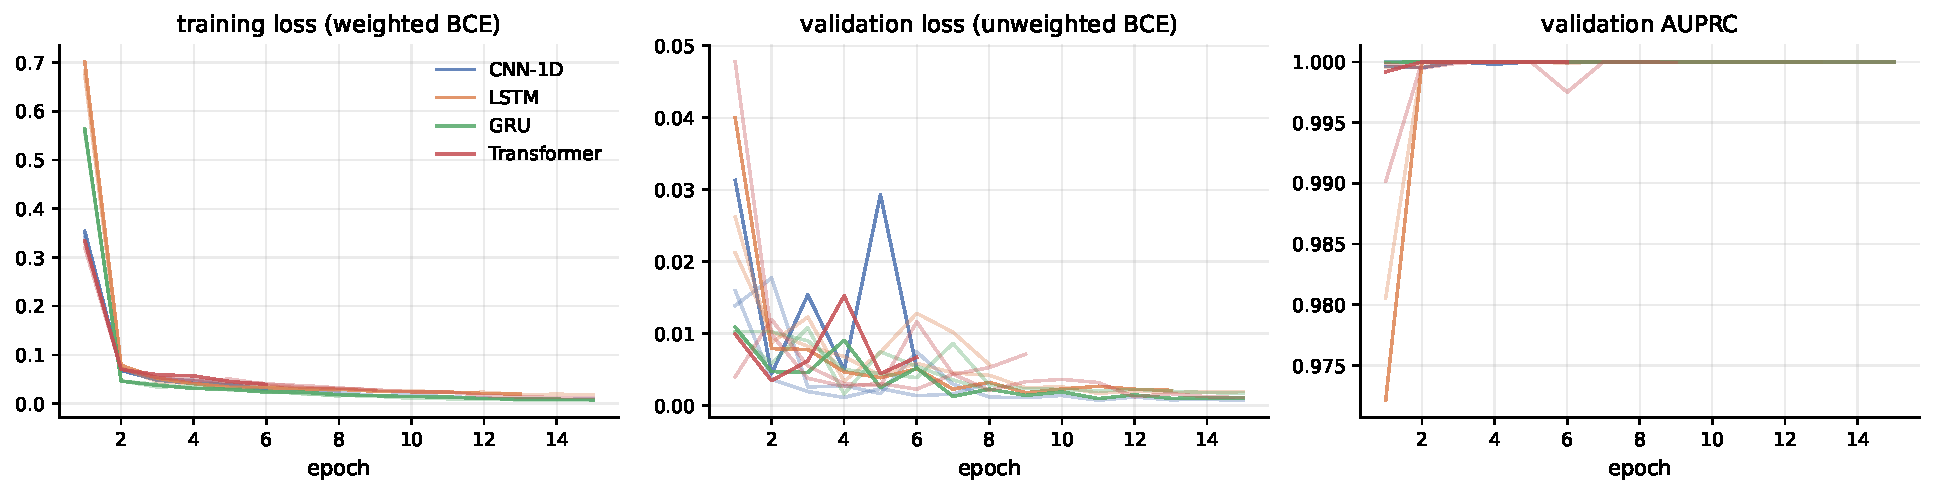
\includegraphics[width=\textwidth]{fig12_learning_curves}
\caption{Learning curves of the final runs (seed 0 opaque, seeds 1--2 transparent).}
\label{fig:curves}
\end{figure}

\begin{figure}[H]
\centering
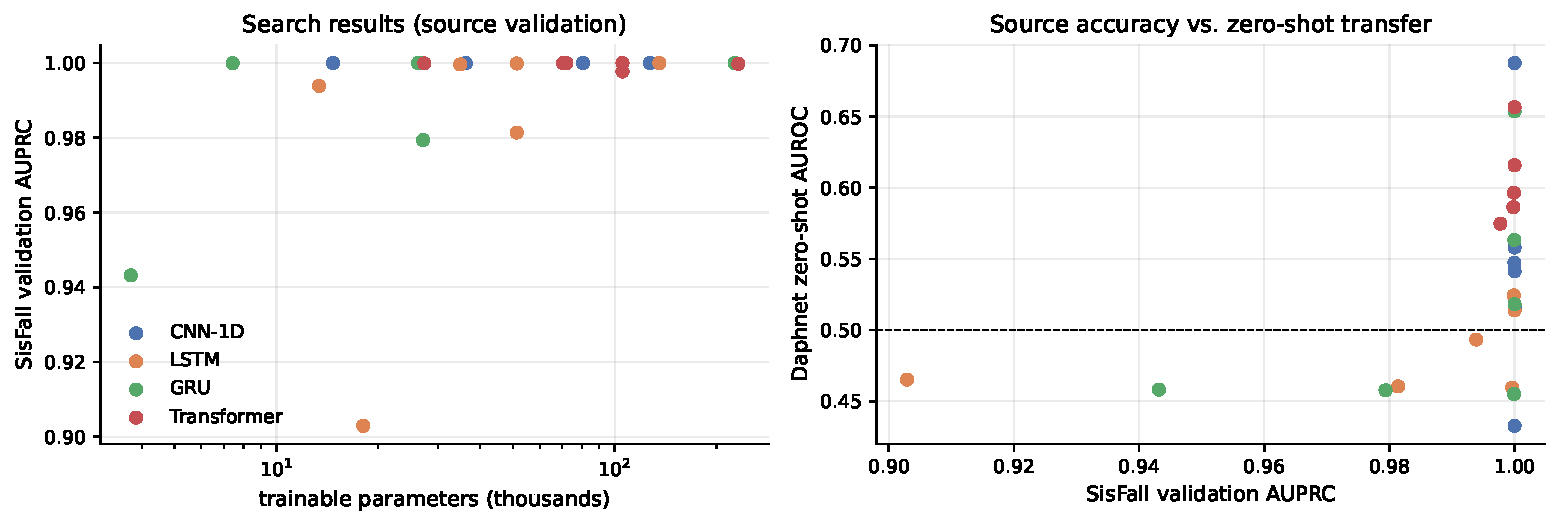
\includegraphics[width=0.95\textwidth]{fig11_hparam_search}
\caption{Hyper-parameter search. Left: validation AUPRC against model size. Right: validation AUPRC
against the Daphnet AUROC that the same configuration would obtain (not used for selection).}
\label{fig:hpsearch}
\end{figure}
